\chapter{\acrshort{wcc} - Proof of concept}\label{prole}
In the context of this research, we have started approaching to the the problem first evaluating the suitability of \acrlong{hs}
to implement the \acrlong{dp}. On the other hand and for test empirically this implementation we develop a Proof of Concept solving 
the \acrlong{wcc} of a Graph using \acrlong{dp} with \acrshort{hs}.
Since we have obtained positive results on this initial research we decided to write a contribution that was accepted and we presented in \acrshort{prole21}~\cite{prole21} 
conference in September of 2021.
In this chapter, we are going to describe the details and results obtained in that contribution that plant the seed for the present work.

\section{Motivation}
Effective streaming processing of large amounts of data has been studied for several years~\cite{enumeratingsg, exploting, onthefly} as a key factor providing fast and incremental 
results in big data algorithmic problems. One of the most explored techniques, regardless of the approach, is the exploitation of parallel techniques to take advantage of the available 
computational power as much as possible. In that regard, the \acrfull{dp} \cite{dpdef} has lately emerged as one of the models that exploit data streaming processing using a dynamic pipeline parallelism approach \cite{onthefly}. 
This computational model has been designed with a functional focus, where the main components of the paradigm are functional stages or pipes which dynamically enlarge and shrink depending on incoming data.  

One of the biggest challenges of implementing a \acrfull{dpf} is to find a proper set of tools and programming language which can take advantage of both of its primary aspects: \begin{inparaenum}[i\upshape)]
\item  \emph{fast parallel} processing and 
\item  \emph{strong theoretical} foundations that manage computations as first-class citizens.
 \end{inparaenum}
\acrfull{hs} is a statically typed pure functional language which has been designed and evolved from its birth in 1987, on strong theoretical foundations where computations are primary entities, 
and at the same time has been providing a powerful set of tools for writing multithreading and parallel programs with optimal performance \cite{parallelbook, monadpar}.

The main objective of this contribution was to explore the feasibility of using a  \acrfull{fp} language to implement a \acrshort{dpf}. In particular, 
we tackle the problem of establishing the basis of an implementation of a \acrshort{dpf}  in \acrshort{hs}, a pure functional language. This is,  our aim is to determine the particular features (i.e., versions and libraries) 
of this language that will allow for an efficient implementation of the \acrshort{dpf}. To be concrete, through a particular and very relevant problem as the computation of the \acrfull{wcc} of a graph,  we study the 
critical features required  in \acrshort{hs} for a \acrshort{dpf} implementation.

\section{Implementation}
Let us consider the problem of computing the (weak) connected components of a graph $G$ using \acrshort{dp}. A connected component of a graph is a subgraph in which any two vertices are connected by paths. Thus, finding connected components of a directed graph implies obtaining the minimal partition of the set of nodes induced by the relationship \textit{connected}, i.e., there is a path between each pair of nodes. The input of the Dynamic Pipeline for computing the WCC of a graph, $\dpwcc$, is a sequence of edges ending with $\eof$%$G=\{(v,w) | v,w\in V, v\neq w\}$, this is a graph given in terms of a stream of edges
\footnote{Note that there are neither isolated vertices nor loops in the source graph $G$.}. The connected components are output as soon as they are computed, i.e., they are produced incrementally. 
%
$\dpwcc$ is defined in terms of the behavior of its four kinds stages: \textit{Source} ($\iwc$),  \textit{Generator} ($\gwc$),  \textit{Sink} ($\owc$), and \textit{Filter}($\fwc$) stages. Additionally,  the channels connecting these stages must be defined. In $\dpwcc$, stages are connected linearly and unidirectionally through the channels $\ice$ and  $\csofv$. Channel $\ice$ carries edges while channel  $\csofv$ conveys sets of connected vertices. Both channels end by the $\eof$ mark. The initial configuration of $\dpwcc$ is $\iwc \:\rightrightarrows\:\gwc \:\rightarrow \: \owc$, where $\rightrightarrows$ represents  channels $\ice$ and $\csofv$ while $\rightarrow$ represents the channel $\csofv$.
 
 Once activated the initial $\dpwcc$, the stream of edges is fed into $\iwc$ and $\owc$ produces the resulting connected components. $\gwc$ has as parameter the template of the stage  $\fwc$. When an edge $(v,w)$ arrives to $\gwc$, it  spawns a new instance of $\fwc$ before $\gwc$. For example, the first time a filter instance is spawned, the $\dpwcc$ evolves to this one: $\iwc \:\rightrightarrows\: \fwc \:\rightrightarrows\: \gwc \:\rightarrow \: \owc$. The state of this new filter instance is initialized with the vertices $\{v,w\}$. When $\eof$ arrives to $\gwc$, it connects previous filter instance to $\owc$ through $\csofv$; then, $\gwc$ dies and the $\dpwcc$ evolves as follows: $\iwc \:\rightrightarrows\: \fwc \:\rightrightarrows\: \cdots \fwc \:\rightrightarrows \: \owc$. The behavior of $\fwc$ is given by a sequence of two actors (scripts). In what follows we denote these actors by $\Act$ and $\Actt$, respectively. The script $\Act$ keeps a set of connected vertices ($CV$) in the state of the $\fwc$ instance. When an edge $e$ arrives, if an endpoint of $e$ is present in the state, then the other endpoint of $e$ added to $CV$.  Edges without incident endpoints are passed to the next stage. When $\eof$ arrives at channel $\ice$, it is passed to the next stage and the script $\Actt$ starts its execution.  If script $\Actt$ receives a set of connected vertices $CV$ in $\csofv$, it determines if the intersection between $CV$ and the nodes in its state is not empty. If so, it adds the nodes in $CV$  to its state. Otherwise, the $CV$ is passed to the next stage.  Whenever $\eof$ is received, $\Actt$ passes--through $\csofv$-- the set of vertices in its state and the $\eof$ mark to the next stage; then, it dies.
 The behavior of $\iwc$ corresponds to  the identity transformation over the data stream of edges.  As edges arrive, they are passed through  $\ice$ to the next stage. When receiving $\eof$ on $\ice$, this mark is put on both channels. Then, $\iwc$ dies. 


\section{Empirical Evaluation}
The empirical study aims at evaluating the performance of $\dpwcc$ when implemented in \acrshort{hs}. 
Our goal is to answer the following research questions: 

\begin{inparaenum}[\bf {\bf RQ}1\upshape)]
\label{res:question}
    \item Does $\dpwcc$ in \acrshort{hs} support the dynamic parallelization level that $\dpwcc$ requires?
    \item Is $\dpwcc$ in \acrshort{hs} competitive compared with default implementations on base libraries for the same problem?
    \item Does $\dpwcc$ in \acrshort{hs} handle memory efficiently?
\end{inparaenum}

We have conducted different kinds of experiments to test our assumptions and verify the correctness of the implementation.
First, we have performed an \emph{Implementation Analysis} in which we have selected some graphs from \acrfull{snap} \cite{stanford} 
and analyze how the implementation behaves under real-world graphs if it timeouts or not and if it is producing correct results in terms of the amount of \acrshort{wcc} that we know beforehand.
We have also tested the implementation doing a \emph{Benchmark Analysis} where we focus on two different types of benchmarks. On the one hand, 
using \texttt{criterion} library \cite{criterion}, we have evaluated a benchmark between our solution and \acrshort{wcc} algorithm implemented in \texttt{containers} \acrshort{hs} library \cite{containers} 
using \mintinline{haskell}{Data.Graph}. On the other hand, we have compared if the results are being generated incrementally in both cases and how that is done during the pipeline execution time. 
This last analysis has been conducted using \texttt{diefpy} tool \cite{diefpaper,diefpy}.
Finally, we have executed a \textit{Performance Analysis} in which we have to gather profiling data from \acrfull{ghc} for one of the real-world graphs, to measure how the program performs 
regarding multithreading and memory allocation.

\paragraph{Implementation analysis} The following represents the execution for running these graphs on our \acrshort{dp} implementation.

\begin{table}[H]
  \centering
  \begin{tabular}{|l|r|r|r|r|}
   \hline
   \textbf{Network} & \textbf{Exec Param} & \textbf{MUT Time} & \textbf{GC Time} & \textbf{Total Time}\\
   \hline
   Enron Emails & \mintinline{bash}{+RTS -N4 -s} & 2.797s & 0.942s & 3.746s \\
   \hline
   Astro Physics Coll Net & \mintinline{bash}{+RTS -N4 -s} & 2.607s & 1.392s & 4.014s \\
   \hline
   Google Web Graph & \mintinline{bash}{+RTS -N8 -s} & 137.127s & 218.913s & \textbf{\textcolor{red}{356.058s}} \\
   \hline
  \end{tabular}
 \caption{Execution times}
 \label{table:5}
 \end{table}

It is important to point out that since the first two networks are smaller in the number of edges compared with \emph{web-Google}, 
executing those with $8$ cores as the \mintinline{bash}{-N} parameters indicates, does not affect the final speed-up since \acrshort{ghc} 
is not distributing threads on extra cores because it handles the load with $4$ cores only.
As we can see in \autoref{table:5}, we are obtaining remarkable execution times for the first two graphs and it seems not to be the case 
for \textit{web-Google} due to the topology of the graph which is much more dense in terms of connected components than the others.

\paragraph{Benchmark Analysis} Regarding mean execution times for each implementation on each case measure by \texttt{criterion} library \cite{criterion}, we can display the following results:

\begin{table}[H]
  \centering
  \begin{tabular}{|l|l|l|l|}
   \hline
   \textbf{Network} & \textbf{\acrshort{dpwcc}} & \textbf{\acrshort{hs} \texttt{containers}} & \textbf{Speed-up}\\
   \hline
   Enron Emails & 4.68s &  6.46s & 1.38\\
   \hline
   Astro Physics Coll Net & 4.98s & 6.95s  & 1.39\\
   \hline
   Google Web Graph & 386s & 106s & 0.27\\
   \hline
  \end{tabular}
 \caption{Mean Execution times}
 \label{table:6}
 \end{table}

These results allow for answering Question [Q2]. where we have seen that the graph topology is affecting the performance and the parallelization, penalizing \acrshort{dpwcc} for this particular case. In this benchmark, 
the solution against a non-parallel \texttt{containers} \mintinline{haskell}{Data.Graph} confirms the hypothesis. 

\paragraph{Diefficency metrics} Some considerations are needed before starting to analyze the data gathered with \acrfull{dm} tool. Firstly, the tool is plotting the results according to the traces generated by the implementation, 
both \acrshort{dpwcc} and \acrshort{hs} \emph{containers}. By the nature of \acrshort{dp} model, we can gather or register that timestamps as long as the model is generating results. In the case of \acrshort{hs} \texttt{containers}, this is not possible since it 
calculates \acrshort{wcc} at once. This is not an issue and we still can check at what point in time all \acrshort{wcc} in \acrshort{hs} \texttt{containers} are generated. In those cases, we are going to see a straight vertical line. 

It is important to remark that we needed to scale the timestamps because we have taken the time in nanoseconds. After all, the incremental generation between one \acrshort{wcc} and the other is very 
small but significant enough to be taken into consideration. Thus, if we left the time scale in integer milliseconds, microseconds, or nanoseconds integer part it cannot be appreciated. In case of escalation, we are discounting 
the nanosecond integer of the first generated results resulting in a time scale that starts close to $0$. This does not mean that the first result is generated at $0$ time, but we are discarding the previous time to focus on how the results are incrementally generated.

Having said that, we can see the results of \acrshort{dm} which are presented in two types of plots. The first one is regular line graphs in where the $x$ axis shows the time escalated when 
the result was generated and the $y$ axis is showing the component number that was generated at that time. The second type of plot is a radar plot in which shows how the solution is behaving 
on the dimensions of  \acrfull{tfft}, \acrfull{et}, \acrfull{tt}, \acrfull{comp} and \acrfull{dt} and how are the tension between them; all these metrics are higher is better. 
All the details about these metrics are explained here \cite{diefpaper}.

\begin{figure}[!htb]
    \centering
    \begin{minipage}{0.33\textwidth}
     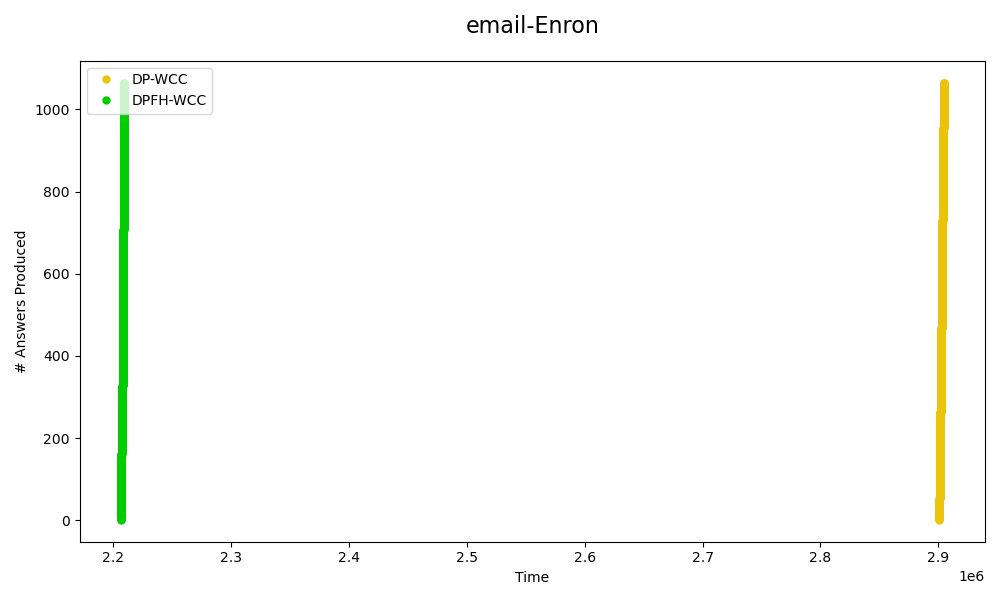
\includegraphics[width=1\linewidth, height=0.2\textheight]{email_enron}
      \caption{email-Enron \acrshort{dm}}
      \label{fig:dief:1}
    \end{minipage}%
    \begin{minipage}{0.33\textwidth}
     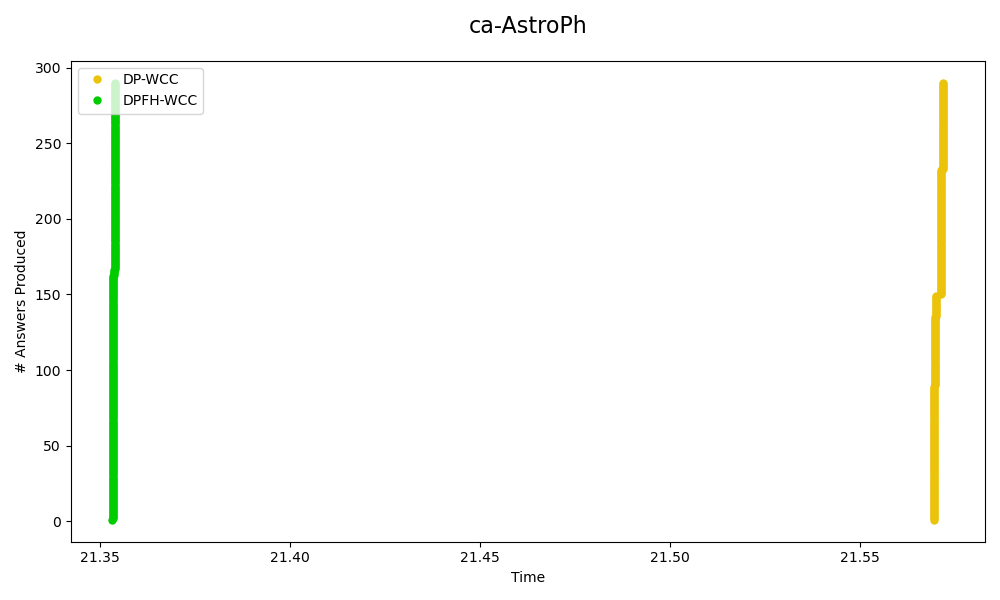
\includegraphics[width=1\linewidth, height=0.2\textheight]{ca_astroph}
      \caption{ca-AstroPh \acrshort{dm}}
      \label{fig:dief:2}
    \end{minipage}%
    \begin{minipage}{0.33\textwidth}
     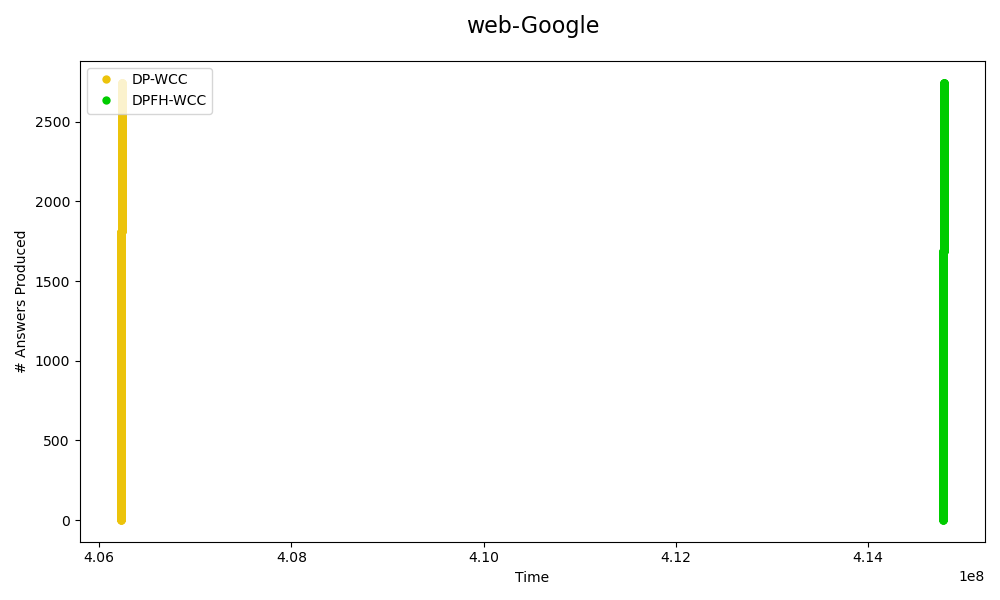
\includegraphics[width=1\linewidth, height=0.2\textheight]{web_google}
      \caption{web-Google \acrshort{dm}}
      \label{fig:dief:3}
    \end{minipage}
\end{figure}

Based on the results shown in all the figures above, all the solutions in \acrshort{dpwcc} are being generated incrementally, 
but there is some difference that we would like to remark. In the case of \emph{email-Enron} and \emph{ca-AstroPh} graphs 
as we can see in \autoref{fig:dief:1} and \autoref{fig:dief:2}, there seems to be a more incremental generation of results. 
This is behavior is measured with the values of \acrfull{dt}. \emph{ca-AstroPh} as it can be seen in \autoref{fig:dief:2}, 
is even more incremental showing a clear separation between some results and others. The \emph{web-Google} network which is 
shown in \autoref{fig:dief:3}, is a little more linear and that is because all the results are being generated with very little 
difference in time between them. Having the biggest \acrshort{wcc} at the end of \emph{web-Google} \acrshort{dp} algorithm 
it is retaining results until the biggest \acrshort{wcc} can be solved, which takes longer. 


\paragraph{Multithreading} For analyzing parallelization and multithreading we have used \textit{ThreadScope} \cite{threadscope} which allows us to see how the parallelization is taking place on \acrshort{ghc} at a fine grained level and how the threads are distributed throughout the different cores requested with the \mintinline{bash}{-N} execution \texttt{ghc-option} flag.
The distribution of the load is more intensive at the end of the execution, where \mintinline{haskell}{actor2} filter stage 
of the algorithm is taking place and different filters are reaching execution of that second actor.
\begin{wrapfigure}{r}{0.5\textwidth}
  \begin{center}
     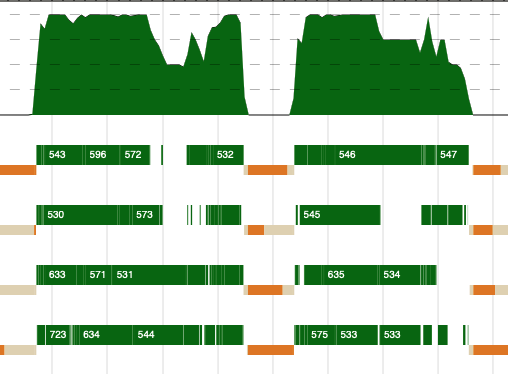
\includegraphics[width=0.48\textwidth, height=0.2\textheight] {screen_2}
    \end{center}
    \captionsetup{type=figure}
    \captionof{figure}{Threadscope Image of Zoomed Fraction}
    \label{fig:4}
 \end{wrapfigure}
~\autoref{fig:4} zooms in on \textit{ThreadScope} output in a particular moment, approximately in the middle of the execution. We can appreciate how many threads are being spawned and by the tool and if they are evenly distributed among cores. The numbers inside green bars represent the number of threads that are being executed on that particular core (horizontal line) at that execution slot. Thus, the number of threads varies among slot execution times because as it is already known, \acrshort{ghc} implements \emph{Preemptive Scheduling} \cite{lightweightghc}.
Having said that, it can be appreciated in \autoref{fig:4} our first assumption that the load is evenly distributed because the mean number of executing threads per core is $571$.

\paragraph{Memory allocation} Another important aspect in our case is how the memory is being managed to avoid memory leaks or other non-desired behavior that increases memory allocation during the execution time. This is even more important in the particular implementation of \acrshort{wcc} using \acrshort{dp} model because it requires to maintain the set of connected components in memory throughout the execution of the program or at least until we can output the calculated \acrshort{wcc} if we reach to the last \textit{Filter} and we know that this \acrshort{wcc} cannot be enlarged anymore.
In order to verify this, we measure memory allocation with \textit{eventlog2html} \cite{eventlog2html} which converts generated profiling memory eventlog files into graphical HTML representation. 
\begin{wrapfigure}{rt!}{0.5\textwidth}
  \begin{center}
     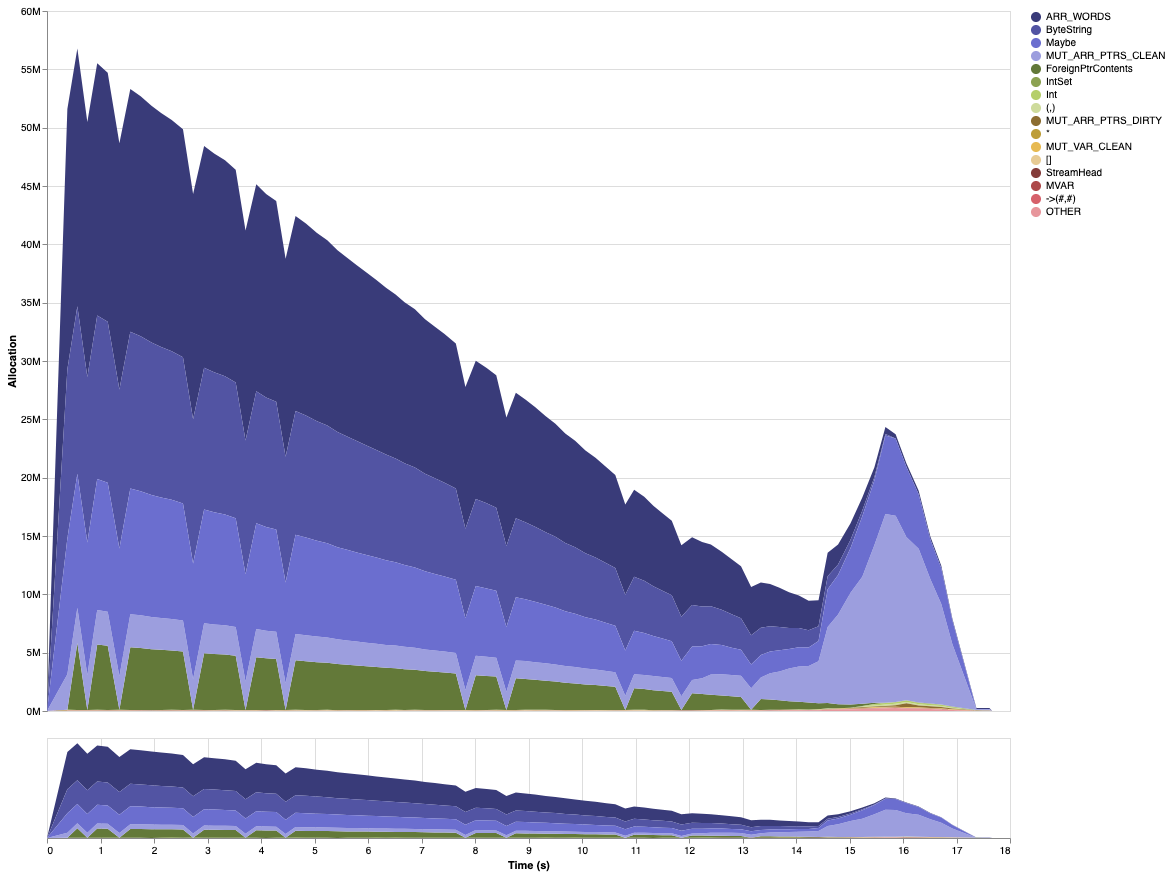
\includegraphics[width=0.48\textwidth, height=0.2\textheight] {visualization}
       \end{center}
     \caption{Memory Allocation}
     \label{fig:5}
 \end{wrapfigure}

As we can see in \autoref{fig:5}, \acrshort{dpwcc} does an efficient work on allocating memory since we are not using more than $57$ MB of memory during the whole execution of the program.
On the other hand, if we analyze how the memory is allocated during the execution of the program, it can also be appreciated that most of the memory is allocated at the beginning of the program and steadily decrease over time with a small peak at the end that does not overpass even half of the initial peak of $57$ MB. The explanation for this behavior is quite straightforward because at the beginning we are reading from the file and transforming a \mintinline{haskell}{ByteString} buffer to \mintinline{haskell}{(Int, Int)} edges. This is seen in the image in which the dark blue that is on top of the area is \mintinline{haskell}{ByteString} allocation. Light blue is allocation of \mintinline{haskell}{Maybe a} type which is the type that is returned by the \textit{Channels} because it can contain a value or not. Data value \mintinline{haskell}{Nothing} is indicating end of the \textit{Channel}. 
Another important aspect is the green area which represents \mintinline{haskell}{IntSet} allocation, which in the case of our program is the data structure that we use to gather the set of vertices that represents a \acrshort{wcc}. This means that the amount of memory used for gathering the \acrshort{wcc} itself is minimum and it is decreasing over time, which is another empirical indication that we are incrementally releasing results to the user. It can be seen as well that as long the green area reduces the lighter blue (\mintinline{haskell}{MUT_ARR_PTRS_CLEAN} \cite{ghcheap}) increases at the same time indicating that the computations for the output (releasing results) is taking place. 
Finally, according to what we have stated above, we can answer the question [Q3] showing that not only memory management was efficient, but at the same time, the memory was not leaking or increasing across the running execution program.

\section{Conclusions}
The empirical evaluation of the \acrshort{dpwcc} implementation to compute weakly connected components of a graph, evidence suitability, 
and robustness to provide a Dynamic Pipeline Framework in that language. Measuring  using \acrshort{dt} metrics 
reveals some advantageous capability of $\dpwcc$ implementation to deliver incremental results compared with default containers library implementation. 
Regarding the main aspects where DPP is strong, i.e. pipeline parallelism and time processing, the $\dpwcc$ performance shows that Haskell 
can deal with the requirements for the \acrshort{wcc} problem without penalizing neither execution time nor memory allocation. 
In particular, the $\dpwcc$ implementation outperforms in those cases where the topology of the graph is more sparse and where the number of 
vertices in the largest \acrshort{wcc} is not big enough. We think this work has gathered enough evidence to show that the implementation 
of Dynamic Pipeline in Haskell Programming Language is feasible. This fact opens a wide range of algorithms to be explored using the 
Dynamic Pipeline Paradigm, supported by purely functional programming language.

\section{Chapter Summary}
In this chapter we have presented an overview of the previous contribution done for \acrshort{prole21}~\cite{prole21} conference, in order to asses the 
feasibility of implementing \acrshort{dp} using \acrshort{hs}. On that sense we presented an overview of the work, the experiments and conclusions.

